\chapter{HPC ranking of big performance tableaux}
\label{sec:11}

\abstract*{To be written.}

\abstract{To be written.}

\section{C-compiled Python modules}
\label{sec:11.1}

The Digraph3 collection provides cythonized \footnote{see https://cython.org/}, i.e. C-compiled and optimised versions of the main python modules for tackling multiple criteria decision problems facing very large sets of decision alternatives ( $> 10000$ ). Such problems appear usually with a combinatorial organisation of the potential decision alternatives, as is frequently the case in bioinformatics for instance. If HPC facilities with nodes supporting numerous cores ($> 20$) and big RAM ($>$ 50GB) are available, ranking up to several millions of alternatives becomes effectively tractable (see [BIS-2016]).

Four cythonized \Digraph modules, prefixed with the letter \texttt{c} and taking a \texttt{pyx} extension, are provided with their corresponding setup tools in the \texttt{cython} directory of the \Digraph resources, namely:
\begin{itemize}
\item[] \texttt{cRandPerfTabs.pyx},
\item[] \texttt{cIntegerOutrankingDigraphs.pyx},
\item[] \texttt{cIntegerSortingDigraphs.pyx}, and
\item[] \texttt{cSparseIntegerOutrankingDigraphs.pyx}.
\end{itemize}

Their automatic compilation and installation, alongside the standard \Digraph python3 modules, requires the \emph{cython} compiler \footnote{see https://cython.org/} ( \texttt{...\$ python3 -m pip install cython} ) and a C compiler (\texttt{...\$ sudo apt install gcc} on Ubuntu).

These cythonized modules, specifically designed for being run on HPC clusters (see \href{https://hpc.uni.lu}{https://hpc.uni.lu}), require the Unix \emph{forking} start method of subprocesses (see start methods of the \href{https://docs.python.org/3/library/multiprocessing.html#contexts-and-start-methods}{multiprocessing library})  and therefore, due to forking problems on Mac OS platforms, may only operate safely on Linux platforms.

\section{Big Data performance tableaux}
\label{sec:11.2}

In order to efficiently type the C variables, the \texttt{cRandPerfTabs} module provides the usual random performance tableau models, but, with \emph{integer} action keys, \emph{float} performance evaluations, \emph{integer} criteria weights and \emph{float} discrimination thresholds. And, to limit as much as possible memory occupation of class instances, all the usual verbose comments are dropped from the description of the \texttt{actions} and \texttt{criteria} dictionaries. 

\begin{lstlisting}[caption={Big data performance tableau format},label=list:11.1]
>>> from cRandPerfTabs import cRandomPerformanceTableau
>>> t = cRandomPerformanceTableau(numberOfActions=4,\
...                               numberOfCriteria=2)
>>> t
  *------- PerformanceTableau instance description ------*
    Instance class   : cRandomPerformanceTableau
    Seed             : None
    Instance name    : cRandomperftab
    Actions          : 4
    Criteria         : 2
    Attributes       : ['randomSeed', 'name', 'actions',
                        'criteria', 'evaluation', 'weightPreorder']
>>> t.actions
   OrderedDict([(1, {'name': '#1'}), (2, {'name': '#2'}),
		(3, {'name': '#3'}), (4, {'name': '#4'})])
>>> t.criteria
   OrderedDict([
   ('g1', {'name': 'RandomPerformanceTableau() instance',
	       'thresholds': {'ind': (10.0, 0.0),
			       'pref': (20.0, 0.0),
			       'veto': (80.0, 0.0)},
	       'scale': (0.0, 100.0),
	       'weight': 1,
	       'preferenceDirection': 'max'}),
   ('g2', {'name': 'RandomPerformanceTableau() instance',
	       'thresholds': {'ind': (10.0, 0.0),
			       'pref': (20.0, 0.0),
			       'veto': (80.0, 0.0)},
	       'scale': (0.0, 100.0),
	       'weight': 1,
	       'preferenceDirection': 'max'})])
>>> t.evaluation
  {'g1': {1: 35.17, 2: 56.4, 3: 1.94, 4: 5.51},
   'g2': {1: 95.12, 2: 90.54, 3: 51.84, 4: 15.42}}
>>> t.showPerformanceTableau()
	Criteria |  'g1'    'g2'   
	Actions  |    1       1    
	---------|---------------
	   '#1'  |  91.18   90.42  
	   '#2'  |  66.82   41.31  
	   '#3'  |  35.76   28.86  
	   '#4'  |   7.78   37.64  
\end{lstlisting}

Conversions from the Big Data model to the standard model and vice versa are provided.

\begin{lstlisting}   
>>> t1 = t.convert2Standard()
>>> t1.convertWeight2Decimal()
>>> t1.convertEvaluation2Decimal()
>>> t1
  *------- PerformanceTableau instance description ------*
   Instance class   : PerformanceTableau
   Seed             : None
   Instance name    : std_cRandomperftab
   Actions          : 4
   Criteria         : 2
   Attributes       : ['name', 'actions', 'criteria',
                       'weightPreorder', 'evaluation',
                       'randomSeed']
\end{lstlisting}

\section{C-implemented integer-valued outranking digraphs}
\label{sec:11.3}


The C compiled version of the bipolar-valued digraph model takes integer relation characteristic values.

\begin{lstlisting}[caption={Constructing big outranking digraphs},label=list:11.2]
>>> t = cRandomPerformanceTableau(numberOfActions=1000,\
...                               numberOfCriteria=2)
>>> from cIntegerOutrankingDigraphs import\
...                 IntegerBipolarOutrankingDigraph
>>> g = IntegerBipolarOutrankingDigraph(t,\
...                 Threading=True, nbrCores=4)
>>> g
  *------- Object instance description ------*
   Instance class   : IntegerBipolarOutrankingDigraph
   Instance name    : rel_cRandomperftab
   Actions          : 1000
   Criteria         : 2
   Size             : 465024
   Determinateness  : 56.877
   Valuation domain : {'min': -2, 'med': 0, 'max': 2,
                       'hasIntegerValuation': True}
   ----  Constructor run times (in sec.) ----
   Total time       : 4.23880
   Data input       : 0.01203
   Compute relation : 3.60788
   Gamma sets       : 0.61889
   Threads          : 4
   Attributes       : ['name', 'actions', 'criteria',
       'totalWeight', 'valuationdomain',
       'methodData', 'evaluation',
       'order', 'runTimes', 'nbrThreads',
       'relation', 'gamma', 'notGamma']
\end{lstlisting}

On a classic intel-i7 equipped PC with four single threaded cores, the\\ \texttt{IntegerBipolarOutrankingDigraph} constructor takes about four seconds for computing a \emph{million} pairwise outranking characteristic values (see Listing \ref{list:11.2}). In a similar setting, the standard \texttt{BipolarOutrankingDigraph} constructor operates more than two times slower.

\begin{lstlisting}
>>> from outrankingDigraphs import BipolarOutrankingDigraph
>>> t1 = t.convert2Standard()
>>> g1 = BipolarOutrankingDigraph(t1,\
...                Threading=True,nbrCores=4)
>>> g1
  *------- Object instance description ------*
    Instance class   : BipolarOutrankingDigraph
    Instance name    : rel_std_cRandomperftab
    Actions        : 1000
    Criteria       : 2
    Size             : 465024
    Determinateness  : 56.817
    Valuation domain : {'min': Decimal('-1.0'),
			'med': Decimal('0.0'),
			'max': Decimal('1.0'),
			'precision': Decimal('0')}
    ----  Constructor run times (in sec.) ----
    Total time       : 8.63340
    Data input       : 0.01564
    Compute relation : 7.52787
    Gamma sets       : 1.08987
    Threads         : 4
\end{lstlisting}

By far, most of the run time is in each case needed for computing the individual pairwise outranking characteristic values. Notice also below the memory occupations of both outranking digraph instances. 

\begin{lstlisting}
>>> from digraphsTools import total_size
>>> total_size(g)
    108662777
>>> total_size(g1)
    212679272
>>> total_size(g1.relation)/total_size(g1)
    0.34
>>> total_size(g1.gamma)/total_size(g1)
    0.45
\end{lstlisting}

About 103MB for $g$ and 202MB for $g1$. The standard \texttt{Decimal} valued \\
\texttt{BipolarOutrankingDigraph} instance $g1$ thus nearly doubles the memory\\ occupation of the corresponding \texttt{IntegerBipolarOutrankingDigraph} $g$ instance (see Line 3 and 5 above). 3/4 of this memory occupation is due to the \texttt{g1.relation} ($34\%$) and the \texttt{g1.gamma} ($45\%$) dictionaries. And these ratios quadratically grow with the digraph order. To limit the object sizes for really big outranking digraphs, we need to abandon the complete implementation of adjacency tables and gamma functions.

\section{The sparse outranking digraph implementation}
\label{sec:11.4}

The idea is to first decompose the complete outranking relation into an ordered collection of equivalent quantile performance classes. Let us consider for this illustration a random performance tableau with 100 decision alternatives evaluated on 7 criteria.

\begin{lstlisting}
>>> from cRandPerfTabs import cRandomPerformanceTableau
>>> t = cRandomPerformanceTableau(numberOfActions=100,\
...                       numberOfCriteria=7,seed=100)
\end{lstlisting}

We sort the 100 decision alternatives into overlapping quartile classes and rank with respect to the average quantile limits.

\begin{lstlisting}[caption={Constructing the sparse integer outranking digraph},label=list:11.3]
>>> from cSparseIntegerOutrankingDigraphs import\
...                    SparseIntegerOutrankingDigraph
>>> sg = SparseIntegerOutrankingDigraph(t,quantiles=4)
>>> sg
  *----- Object instance description --------------*
   Instance class    : SparseIntegerOutrankingDigraph
   Instance name     : cRandomperftab_mp
   Actions           : 100
   Criteria          : 7
   Sorting by        : 4-Tiling
   Ordering strategy : average
   Ranking rule      : Copeland
   Components        : 6
   Minimal order     : 1
   Maximal order     : 35
   Average order     : 16.7
   fill rate         : 24.970%
  *----  Constructor run times (in sec.) ----
   Nbr of threads    : 1
   Total time        : 0.08212
   QuantilesSorting  : 0.01481
   Preordering       : 0.00022
   Decomposing       : 0.06707
   Ordering          : 0.00000
   Attributes       : ['runTimes', 'name', 'actions',
       'criteria', 'evaluation', 'order', 'dimension',
       'sortingParameters', 'nbrOfCPUs',
       'valuationdomain', 'profiles', 'categories',
       'sorting', 'minimalComponentSize',
       'decomposition', 'nbrComponents', 'nd',
       'components', 'fillRate',
       'maximalComponentSize', 'componentRankingRule',
       'boostedRanking']
\end{lstlisting}

We obtain in this example here a decomposition into 6 linearly ordered components with a maximal component size of 35 for component $c3$.

\begin{lstlisting}
>>> sg.showDecomposition()
 *--- quantiles decomposition in decreasing order---*
  c1. ]0.75-1.00] : [3,22,24,34,41,44,50,53,56,62,93]
  c2. ]0.50-1.00] : [7,29,43,58,63,81,96]
  c3. ]0.50-0.75] : [1,2,5,8,10,11,20,21,25,28,30,33,
                     35,36,45,48,57,59,61,65,66,68,70,
                     71,73,76,82,85,89,90,91,92,94,95,97]
  c4. ]0.25-0.75] : [17,19,26,27,40,46,55,64,69,87,98,100]
  c5. ]0.25-0.50] : [4,6,9,12,13,14,15,16,18,23,31,32,
                     37,38,39,42,47,49,51,52,54,60,67,72,
                     74,75,77,78,80,86,88,99]
  c6. ]<-0.25]    : [79,83,84]
\end{lstlisting}

A restricted outranking relation is stored for each component with more than one alternative. The resulting global relation map of the first ranked 75 alternatives looks as follows.

\begin{lstlisting}
>>> sg.showRelationMap(toIndex=75)
\end{lstlisting}  

\begin{figure}[h]
\sidecaption
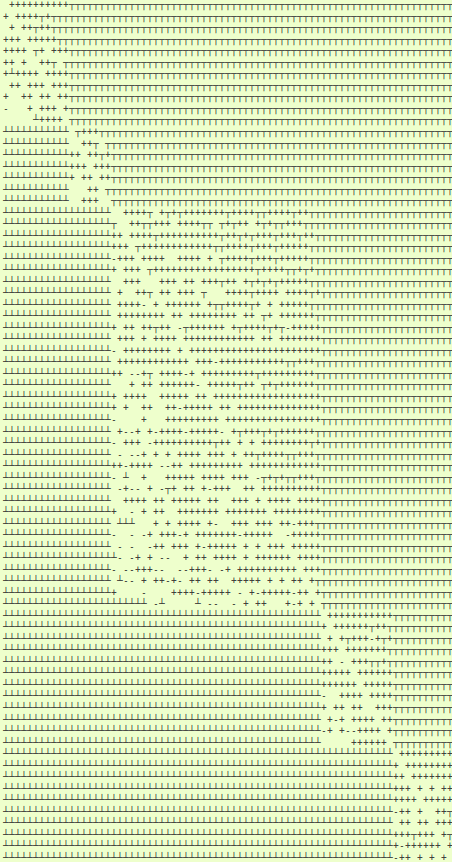
\includegraphics[width=7cm]{Figures/sparseRelationMap.png}
\caption{Sparse quartiles-sorting decomposed outranking relation (extract). \textbf{Legend}: \emph{outranking} for certain ($\top$); \emph{outranked} for certain ($\bot$); more or less \emph{outranking} ($+$); more or less \emph{outranked} ($-$); \emph{indeterminate} (\ ).
}
\label{fig:11.1}       % Give a unique label
\end{figure}
\clearpage

With a fill rate of $25\%$, the memory occupation of this sparse outranking digraph $sg$ instance takes now only 769kB, compared to the 1.7MB required by a corresponding standard \texttt{BipolarOutrankingDigraph} instance (see Listing \ref{list:113}).

\begin{lstlisting}
>>> print('%.0fkB' % (total_size(sg)/1024) )
    769kB
\end{lstlisting}

For sparse outranking digraphs, the adjacency table is implemented as a dynamic \texttt{relation()} function instead of a double dictionary.

\begin{lstlisting}[caption={The \texttt{relation()} function of a sparse outranking digraph},label=list:11.4,basicstyle=\scriptsize]
   def relation(self, int x, int y):
       """
       *Parameters*:
           * x (int action key),
           * y (int action key).
       Dynamic construction of the global outranking
       characteristic function *r(x S y)*.
       """
       cdef int Min, Med, Max, rx, ry
       Min = self.valuationdomain['min']
       Med = self.valuationdomain['med']
       Max = self.valuationdomain['max']
       if x == y:
           return Med
       cx = self.actions[x]['component']
       cy = self.actions[y]['component']
       #print(self.components)
       rx = self.components[cx]['rank']
       ry = self.components[cy]['rank']
       if rx == ry:
           try:
               rxpg = self.components[cx]['subGraph'].relation
               return rxpg[x][y]
           except AttributeError:
               componentRanking = self.components[cx]['componentRanking']
               if componentRanking.index(x) < componentRanking.index(x):
                   return Max
               else:
                   return Min
       elif rx > ry:
           return Min
       else:
           return Max
\end{lstlisting}

\section{Ranking big performance tableaux}
\label{sec:12.5}

We may now rank the complete set of 100 decision alternatives by locally ranking with the \Copeland or the \NetFlows rule, for instance, all these individual components.

\begin{lstlisting}
   >>> sg.boostedRanking
    [22, 53, 3, 34, 56, 62, 24, 44, 50, 93, 41, 63, 29, 58,
     96, 7, 43, 81, 91, 35, 25, 76, 66, 65, 8, 10, 1, 11, 61,
     30, 48, 45, 68, 5, 89, 57, 59, 85, 82, 73, 33, 94, 70,
     97, 20, 92, 71, 90, 95, 21, 28, 2, 36, 87, 40, 98, 46, 55,
     100, 64, 17, 26, 27, 19, 69, 6, 38, 4, 37, 60, 31, 77, 78,
     47, 99, 18, 12, 80, 54, 88, 39, 9, 72, 86, 42, 13, 23, 67,
     52, 15, 32, 49, 51, 74, 16, 14, 75, 79, 83, 84]
\end{lstlisting}

When actually computing linear rankings of a set of alternatives, the local outranking relations are of no practical usage, and we may furthermore reduce the memory occupation of the resulting digraph by
\begin{enumerate}
\item refining the ordering of the quantile classes by taking into account how well an alternative is outranking the lower limit of its quantile class, respectively the upper limit of its quantile class is \emph{not} outranking the alternative;
\item dropping the local outranking digraphs and keeping for each quantile class only a locally ranked list of alternatives.
\end{enumerate}
We provide therefore the \texttt{cQuantilesRankingDigraph} class.

\begin{lstlisting}[caption={Ranking the sparse integer outranking digraph},label=list:11.5]
>>> from cSparseIntegerOutrankingDigraphs import\
...           cQuantilesRankingDigraph
>>> qr = cQuantilesRankingDigraph(t,4)
>>> qr
 *----- Object instance description --------------*
  Instance class    : cQuantilesRankingDigraph
  Instance name     : cRandomperftab_mp
  Actions           : 100
  Criteria          : 7
  Sorting by        : 4-Tiling
  Ordering strategy : optimal
  Ranking rule      : Copeland
  Components        : 47
  Minimal order     : 1
  Maximal order     : 10
  Average order     : 2.1
  fill rate         : 2.566%
 *----  Constructor run times (in sec.) ----*
  Nbr of threads    : 1
  Total time        : 0.03702
  QuantilesSorting  : 0.01785
  Preordering       : 0.00022
  Decomposing       : 0.01892
  Attributes       : ['runTimes', 'name',
  'actions', 'order', 'dimension', 'sortingParameters',
  'nbrOfCPUs','valuationdomain', 'profiles', 'categories',
  'sorting', 'minimalComponentSize','decomposition',
  'nbrComponents', 'nd', 'components', 'fillRate',
  'maximalComponentSize', 'componentRankingRule', 'boostedRanking']
\end{lstlisting}

With this \emph{optimised} quantile ordering strategy, we obtain now 47 performance equivalence classes (see Listing \ref{list:11.5} Line 13)

\begin{lstlisting}
>>> qr.components
    OrderedDict([
    ('c01', {'rank': 1,
	     'lowQtileLimit': ']0.75',
	     'highQtileLimit': '1.00]',
	     'componentRanking': [53]}),
    ('c02', {'rank': 2,
	     'lowQtileLimit': ']0.75',
	     'highQtileLimit': '1.00]',
	     'componentRanking': [3, 23, 63, 50]}),
    ('c03', {'rank': 3,
	     'lowQtileLimit': ']0.75',
	     'highQtileLimit': '1.00]',
	     'componentRanking': [34, 44, 56, 24, 93, 41]}), 
    ...
    ...
    ...
    ('c45', {'rank': 45,
	     'lowQtileLimit': ']0.25',
	     'highQtileLimit': '0.50]',
	     'componentRanking': [49]}),
    ('c46', {'rank': 46,
	     'lowQtileLimit': ']0.25',
	     'highQtileLimit': '0.50]',
	     'componentRanking': [52, 16, 86]}),
    ('c47', {'rank': 47,
	     'lowQtileLimit': ']<',
	     'highQtileLimit': '0.25]',
	     'componentRanking': [79, 83, 84]})])
>>> print('%.0fkB' % (total_size(qr)/1024) )
    208kB
\end{lstlisting}

We observe in the Listing above an even more considerably less voluminous memory occupation: 208kB compared to the 769kB of the \texttt{SparseIntegerOutrankingDigraph} instance. It is opportune, however, to measure the loss of quality of the resulting \Copeland ranking when working with sparse outranking digraphs.

.. code-block:: pycon
   :linenos:
\begin{lstlisting}[caption={Measuring the loss of quality with respect to the standard outranking digraph},label=list:11.6]
>>> from cIntegerOutrankingDigraphs import *
>>> ig = IntegerBipolarOutrankingDigraph(t)
>>> print('Complete outranking : %+.4f'\
...  % (ig.computeOrderCorrelation(\
...     ig.computeCopelandOrder())['correlation']))
    Complete outranking : +0.7474

>>> print('Sparse 4-tiling : %+.4f'\
...  % (ig.computeOrderCorrelation(\
...     list(reversed(sg.boostedRanking)))\
...     ['correlation']))   
    Sparse 4-tiling          : +0.7172

>>> print('Optimzed sparse 4-tiling: %+.4f'\
...  % (ig.computeOrderCorrelation(\
...     list(reversed(qr.boostedRanking)))\
...     ['correlation']))  
    Optimzed sparse 4-tiling: +0.7051
\end{lstlisting}

The best ranking correlation with the pairwise outranking situations ($+0.75$) is naturally given when we apply the \Copeland rule to the complete outranking digraph (see Listing \ref{list:10.6} Line 6). When we apply the same rule to the sparse 4-tiled outranking digraph, we get a correlation of $+0.72$ (Line 12), and when applying the \Copeland rule to the optimised 4-tiled digraph, we still obtain a correlation of $+0.71$ (Line 18). These results actually depend on the number of quantiles we use as well as on the given model of random performance tableau.

In case of \texttt{Random3ObjectivesPerformanceTableau} instances, for instance, we would get in a similar setting a complete outranking correlation of $+0.86$, a sparse 4-tiling correlation of $+0.82$, and an optimzed sparse 4-tiling correlation of $+0.81$.

\section{HPC quantiles ranking records}
\label{sec:12.6}

Following from the separability property of the $q$-tiles sorting of each action into each $q$-tiles class, the $q$-sorting algorithm may be safely split into as much threads as are multiple processing cores available in parallel. Furthermore, the ranking procedure being local to each diagonal component, these procedures may as well be safely processed in parallel threads on each component restricted outrankingdigraph.

Using the HPC platform of the University of Luxembourg (\href{https://hpc.uni.lu/}{https://hpc.uni.lu/}), the following run times for very big ranking problems could be achieved both:
\begin{itemize}
\item on Iris -skylake nodes with 28 cores \footnote{See https://hpc.uni.lu/systems/iris/}, and
\item on the 3TB -bigmem Gaia-183 node with 64 cores \footnote{See https://hpc.uni.lu/systems/gaia/},
\end{itemize}
by running the cythonized python modules in an Intel compiled virtual Python 3.6.5 environment [GCC Intel(R) 17.0.1 –enable-optimizations c++ gcc 6.3 mode] on Debian 8 Linux.

\begin{figure}[h]
\sidecaption
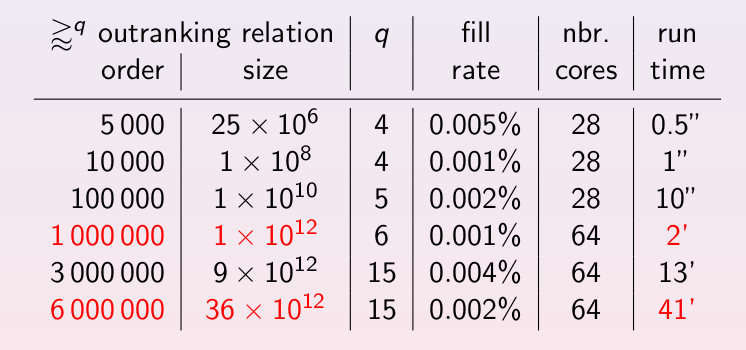
\includegraphics[width=7cm]{Figures/rankingRecords.png}
\caption{HPC-UL Ranking Performance Records (Spring 2018). On the big memory equipped Gaia-183 node, we were able to rank a million decision alternatives in about 2 minutes. We even could linearly rank up to 6 million decision alternatives in about 40 minutes.}
\label{fig:11.2}       % Give a unique label
\end{figure}
  
% Example python session on the HPC-UL Iris-126 -skylake node [7]_

% ..
%    .. figure:: HPC-UniLu-Session.png
%       :width: 500 px
%       :align: center

%    HPC-UL Session (Spring 2018)

% .. code-block:: bash
%    :linenos:

% 	(myPy365ICC) [rbisdorff@iris-126 Test]$ python
% 	Python 3.6.5 (default, May  9 2018, 09:54:28) 
% 	[GCC Intel(R) C++ gcc 6.3 mode] on linux
% 	Type "help", "copyright", "credits" or "license" for more information.
% 	>>>

% .. code-block:: pycon
%    :linenos:

%    >>> from cRandPerfTabs import\
%    ...    cRandom3ObjectivesPerformanceTableau as cR3ObjPT

%    >>> pt = cR3ObjPT(numberOfActions=1000000,\
%    ...             numberOfCriteria=21,\
%    ...             weightDistribution='equiobjectives',\
%    ...             commonScale = (0.0,1000.0),\
%    ...             commonThresholds = [(2.5,0.0),(5.0,0.0),(75.0,0.0)],\
%    ...             commonMode = ['beta','variable',None], \
%    ...             missingDataProbability=0.05,\
%    ...             seed=16)

%    >>> import cSparseIntegerOutrankingDigraphs as iBg
%    >>> qr = iBg.cQuantilesRankingDigraph(pt,quantiles=10,\
%    ...               quantilesOrderingStrategy='optimal',\
%    ...               minimalComponentSize=1,\
%    ...               componentRankingRule='NetFlows',\
%    ...               LowerClosed=False,\
%    ...               Threading=True,\
%    ...               tempDir='/tmp',\
%    ...               nbrOfCPUs=28)

%    >>> qr
%     *----- Object instance description --------------*
%     Instance class    : cQuantilesRankingDigraph
%     Instance name     : random3ObjectivesPerfTab_mp
%     # Actions         : 1000000
%     # Criteria        : 21
%     Sorting by        : 10-Tiling
%     Ordering strategy : optimal
%     Ranking rule      : NetFlows
%     # Components      : 233645
%     Minimal order     : 1
%     Maximal order     : 153
%     Average order     : 4.3
%     fill rate         : 0.001%
%     *----  Constructor run times (in sec.) ----*
%     Nbr of threads    : 28
%     Total time        : 177.02770
%     QuantilesSorting  : 99.55377
%     Preordering       : 5.17954
%     Decomposing       : 72.29356

% On this 2x14c Intel Xeon Gold 6132 @ 2.6 GHz equipped HPC node with 132GB RAM [7]_, deciles sorting and locally ranking a **million** decision alternatives evaluated on 21 incommensurable criteria, by balancing an economic, an environmental and a societal decision objective, takes us about **3 minutes** (see Lines 37-42 above); with 1.5 minutes for the deciles sorting and, a bit more than one minute, for the local ranking of the individual components. 

% The optimised deciles sorting leads to 233645 components (see Lines 32-36 above) with a maximal order of 153. The fill rate of the adjacency table is reduced to 0.001%. Of the potential trillion (10^12) pairwise outrankings, we effectively keep only 10 millions (10^7). This high number of components results from the high number of involved performance criteria (21), leading in fact to a very refined epistemic discrimination of majority outranking margins. 

% A non-optimised deciles sorting would instead give at most 110 components with inevitably very big intractable local digraph orders. Proceeding with a more detailed quantiles sorting, for reducing the induced decomposing run times, leads however quickly to intractable quantiles sorting times. A good compromise is given when the quantiles sorting and decomposing steps show somehow equivalent run times; as is the case in our example session: 99.6 versus 77.3 seconds (see Lines 40 and 42 above).     

% Let us inspect the 21 marginal performances of the five best-ranked alternatives listed below. 

% .. code-block:: pycon
%    :linenos:

%    >>> pt.showPerformanceTableau(\
%    ...               actionsSubset=qr.boostedRanking[:5],\
%    ...               Transposed=True)
   
%    *----  performance tableau -----*
%     criteria | weights |  #773909  #668947  #567308  #578560  #426464
%     ---------|-------------------------------------------------------
%      'Ec01'  |    42   |   969.81   844.71   917.00     NA     808.35  
%      'So02'  |    48   |     NA     891.52   836.43     NA     899.22  
%      'En03'  |    56   |   687.10     NA     503.38   873.90     NA  
%      'So04'  |    48   |   455.05   845.29   866.16   800.39   956.14  
%      'En05'  |    56   |   809.60   846.87   939.46   851.83   950.51  
%      'Ec06'  |    42   |   919.62   802.45   717.39   832.44   974.63  
%      'Ec07'  |    42   |   889.01   722.09   606.11   902.28   574.08  
%      'So08'  |    48   |   862.19   699.38   907.34   571.18   943.34  
%      'En09'  |    56   |   857.34   817.44   819.92   674.60   376.70  
%      'Ec10'  |    42   |     NA     874.86     NA     847.75   739.94  
%      'En11'  |    56   |     NA     824.24   855.76     NA     953.77  
%      'Ec12'  |    42   |   802.18   871.06   488.76   841.41   599.17  
%      'En13'  |    56   |   827.73   839.70   864.48   720.31   877.23  
%      'So14'  |    48   |   943.31   580.69   827.45   815.18   461.04  
%      'En15'  |    56   |   794.57   801.44   924.29   938.70   863.72  
%      'Ec16'  |    42   |   581.15   599.87   949.84   367.34   859.70  
%      'So17'  |    48   |   881.55   856.05     NA     796.10   655.37  
%      'Ec18'  |    42   |   863.44   520.24   919.75   865.14   914.32  
%      'So19'  |    48   |     NA       NA       NA     790.43   842.85  
%      'Ec20'  |    42   |   582.52   831.93   820.92   881.68   864.81  
%      'So21'  |    48   |   880.87     NA     628.96   746.67   863.82  

% The given ranking problem involves 8 criteria assessing the economic performances, 7 criteria assessing the societal performances and 6 criteria assessing the environmental performances of the decision alternatives. The sum of criteria significance weights (336) is the same for all three decision objectives. The five best-ranked alternatives are, in decreasing order: #773909, #668947, #567308, #578560 and #426464.

% Their random performance evaluations were obviously drawn on all criteria with a *good* (+) performance profile, i.e. a Beta(*alpha* = 5.8661, *beta* = 2.62203) law (see the tutorial :ref:`generating random performance tableaux <RandomPerformanceTableau-Tutorial-label>`). 

% .. code-block:: pycon
%    :linenos:

%    >>> for x in qr.boostedRanking[:5]:
%    ...     print(pt.actions[x]['name'],\
%    ...           pt.actions[x]['profile'])
   
%     #773909 {'Eco': '+', 'Soc': '+', 'Env': '+'}
%     #668947 {'Eco': '+', 'Soc': '+', 'Env': '+'}
%     #567308 {'Eco': '+', 'Soc': '+', 'Env': '+'}
%     #578560 {'Eco': '+', 'Soc': '+', 'Env': '+'}
%     #426464 {'Eco': '+', 'Soc': '+', 'Env': '+'}

% We consider now a partial performance tableau *best10*, consisting only, for instance, of the **ten best-ranked alternatives**, with which we may compute a corresponding integer outranking digraph valued in the range (-1008, +1008).  

% .. code-block:: pycon
%    :linenos:

%    >>> best10 = cPartialPerformanceTableau(pt,qr.boostedRanking[:10])
%    >>> from cIntegerOutrankingDigraphs import *   
%    >>> g = IntegerBipolarOutrankingDigraph(best10)
%    >>> g.valuationdomain
%     {'min': -1008, 'med': 0, 'max': 1008, 'hasIntegerValuation': True}
%    >>> g.showRelationTable(ReflexiveTerms=False)
%     * ---- Relation Table -----
%      r(x>y) | #773909 #668947 #567308 #578560 #426464 #298061 #155874 #815552 #279729 #928564
%     --------|-----------------------------------------------------------------------------------
%     #773909 |    -      +390     +90    +270     -50    +340    +220     +60    +116    +222
%     #668947 |    +78     -       +42    +250     -22    +218     +56    +172     +74     +64
%     #567308 |    +70    +418     -      +180    +156    +174    +266     +78    +256    +306
%     #578560 |     -4     +78     +28     -       -12    +100     -48    +154    -110     -10
%     #426464 |   +202    +258    +284    +138     -      +416    +312    +382    +534    +278
%     #298061 |    -48     +68    +172     +32     -42      -      +54     +48    +248    +374
%     #155874 |    +72    +378    +322    +174    +274    +466     -      +212    +308    +418
%     #815552 |    +78    +126    +272    +318     +54    +194    +172     -       -14     +22
%     #279729 |   +240    +230    -110    +290     +72    +140    +388     +62     -      +250
%     #928564 |    +22    +228     -14    +246     +36     +78     +56    +110    +318     -
%     r(x>y) image range := [-1008;+1008]
%    >>> g.condorcetWinners()
%     [155874, 426464, 567308]
%    >>> g.computeChordlessCircuits()
%     []
%    >>> g.computeTransitivityDegree()
%     0.78

% Three alternatives -#155874, #426464 and #567308- qualify as Condorcet winners, i.e. they each **positively outrank** all the other nine alternatives. No chordless outranking circuits are detected, yet the transitivity of the apparent outranking relation is not given. And, no clear ranking alignment hence appears when inspecting the *strict* outranking digraph (i.e. the codual ~(-*g*) of *g*) shown in :numref:`converse-dual_rel_best10`.
  
% .. code-block:: pycon
%    :linenos:

%    >>> (~(-g)).exportGraphViz()
%    *---- exporting a dot file for GraphViz tools ---------*
%     Exporting to converse-dual_rel_best10.dot
%     dot -Tpng converse-dual_rel_best10.dot -o converse-dual_rel_best10.png

% .. figure:: converse-dual_rel_best10.png
%    :name: converse-dual_rel_best10
%    :width: 400 px
%    :align: center

%    Validated *strict* outranking situations between the ten best-ranked alternatives

% Restricted to these ten best-ranked alternatives, the *Copeland*, the *NetFlows* as well as the *Kemeny* ranking rule will all rank alternative #426464 first and alternative #578560 last. Otherwise the three ranking rules produce in this case more or less different rankings.

% .. code-block:: pycon
%    :linenos:

%    >>> g.computeCopelandRanking()
%     [426464, 567308, 155874, 279729, 773909, 928564, 668947, 815552, 298061, 578560]
%    >>> g.computeNetFlowsRanking()
%     [426464, 155874, 773909, 567308, 815552, 279729, 928564, 298061, 668947, 578560]
%    >>> from linearOrders import *
%    >>> ke = KemenyOrder(g,orderLimit=10)
%    >>> ke.kemenyRanking
%     [426464, 773909, 155874, 815552, 567308, 298061, 928564, 279729, 668947, 578560]

% .. note::

%    It is therefore *important* to always keep in mind that, based on pairwise outranking situations, there **does not exist** any **unique optimal ranking**; especially when we face such big data problems. Changing the number of quantiles, the component ranking rule, the optimised quantile ordering strategy, all this will indeed produce, sometimes even substantially, diverse global ranking results. 
 
